\section{Ethylene carbonate with Na/Li TFSI salt}
\label{section:carbonates-spectra}

In this section spectra obtained from AIMD simulations for systems based on EC and its fluorinated derivatives, structural properties of which were described in section~\ref{section:carbonates-structural}, are presented. These results were published in the article~\cite{carbonates}.

\begin{figure}[ht]
    \centering
    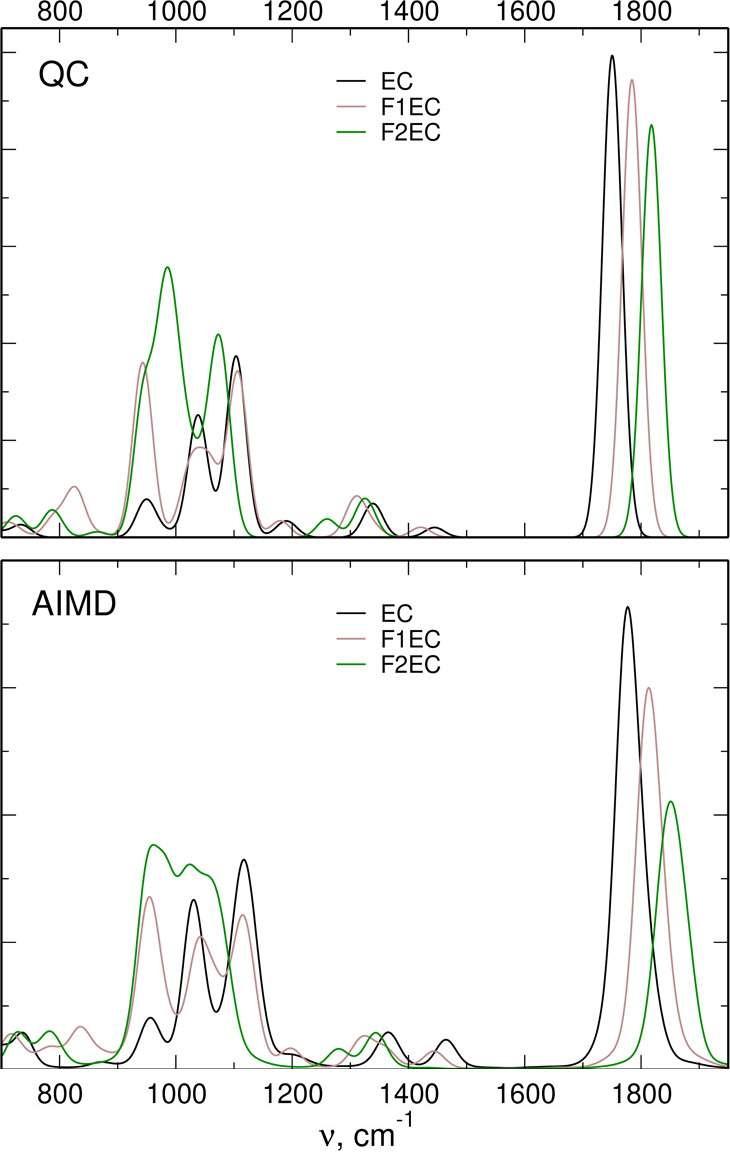
\includegraphics[width=0.4\textwidth]{img/4-ir-spectra-from-aimd-simulations/3-carbonates/ir-neat-solvents.png}
    \caption{Infrared spectra for neat carbonates obtained from QC calculations or from AIMD simulations}
    \label{fig:carbonates-ir-neat-solvents}
\end{figure}

Figure~\ref{fig:carbonates-ir-neat-solvents} presents IR spectra obtained for neat solvents from AIMD simulations, QC results are shown for comparison. For both cases, growing fluorination of the EC leads to increase of the C=O stretching frequency. In QC it changes from 1750~cm$^{-1}$ for EC and 1784~cm$^{-1}$ for F1EC to 1818~cm$^{-1}$ for F2EC. In AIMD results higher frequency values were observed: 1777~cm$^{-1}$ for EC, 1813~cm$^{-1}$ for F1EC and 1851~cm$^{-1}$ for F2EC. Despite the different positions of bands in spectra obtained in QC and AIMD, differences between carbonates with a~different number of fluorine atoms are similar in both approaches.

\begin{figure}[ht]
    \centering
    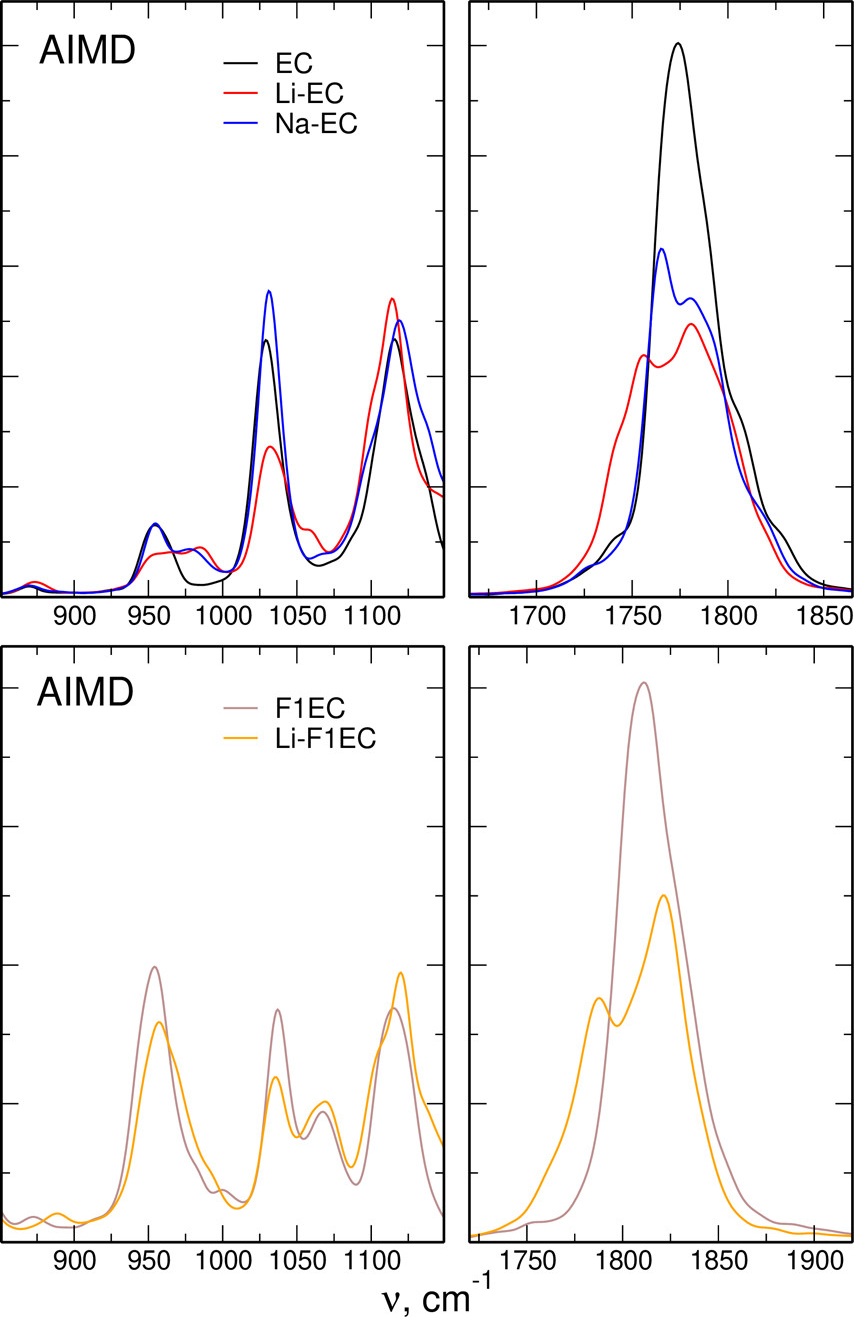
\includegraphics[width=0.4\textwidth]{img/4-ir-spectra-from-aimd-simulations/3-carbonates/ir-electrolytes.png}
    \caption{Infrared spectra of solvents and electrolyte solutions}
    \label{fig:carbonates-ir-electrolytes}
\end{figure}

Next, Figure~\ref{fig:carbonates-ir-electrolytes} shows the spectra for electrolytes, with data for neat solvents shown for comparison. In solutions of MeTFSI salts a~new peak develops near the C=O band at lower frequencies. The biggest shift of this peak is observed for the case of LiTFSI in F1EC (33~cm$^{-1}$), for LiTFSI in EC it is smaller (25~cm$^{-1}$) and the smallest effect is for NaTFSI in EC (16~cm$^{-1}$) but still remarkable. QC calculations identified the vibration ar 850~cm$^{-1}$ as ring breathing mode in solvent molecule. It has very low intensity, but for lithium electrolytes a~small shift towards higher frequencies could be observed, the most visible it is for LiTFSI in F1EC, the maximum is blueshifted by 17~cm$^{-1}$ in comparison with neat F1EC. Another band identified by QC calculations is C-C stretching at about 950~cm$^{-1}$. For electrolytes with EC as the solvent, this peak becomes broader with its barycenter shifted towards higher energies with respect to neat EC. Its intensity is bigger in the F1EC spectrum and in the LiTFSI in F1EC electrolyte a~blue shift by 3~cm$^{-1}$ is observed.

\begin{figure}[ht]
    \centering
    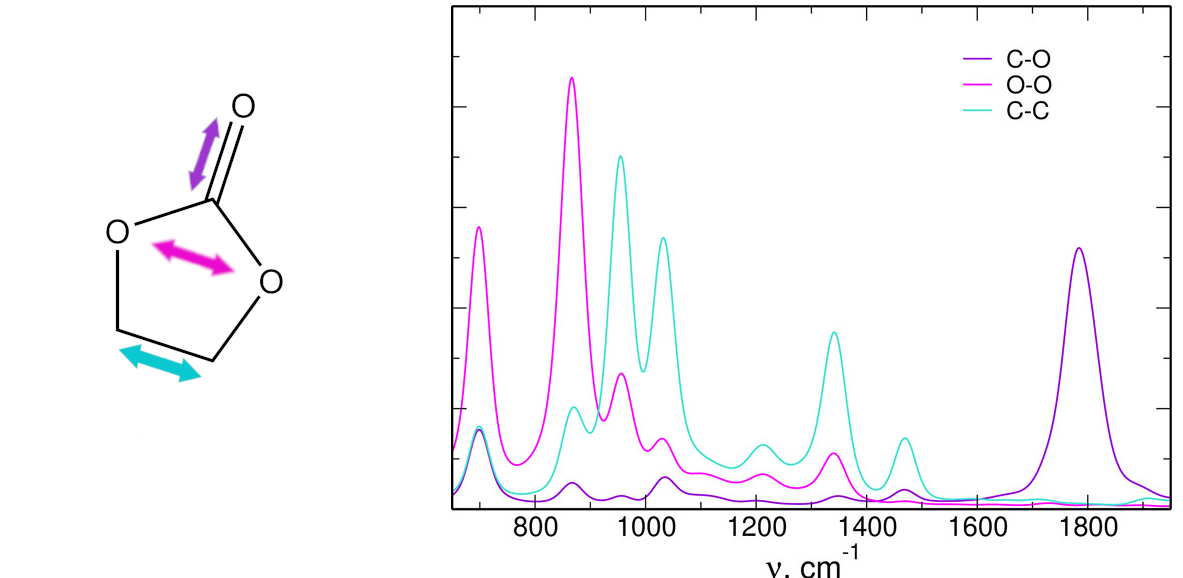
\includegraphics[width=0.6\textwidth]{img/4-ir-spectra-from-aimd-simulations/3-carbonates/ft-carbonates-arrows.png}    
    \singlespacing
    \caption{Power spectrum obtained from Fourier transforms of interatomic distances for EC (right), used atoms/bonds for calculation of these transforms (left), colors correspond to these in Fourier transforms}
    \label{fig:carbonates-ft-carbonates}
\end{figure}

Appearance of new bands or shifts of existing bands in the IR spectra are attributed to interactions between carbonate molecules and Me$^{+}$ cations which affect vibrational frequencies of solvent molecules in the solvation shell of the cation. In Figure~\ref{fig:carbonates-ft-carbonates} FTs of interatomic distances averaged over all molecules for EC are presented. It is clear from this picture that C=O oscillations have frequency close to 1800~cm$^{-1}$, O-O oscillations corresponding to ring breathing mode appear at 850~cm$^{-1}$ and C-C bond stretch at about 950~cm$^{-1}$ and above 1000~cm$^{-1}$, as expected on the basis of the QC calculations.

\begin{figure}[H]
    \centering
    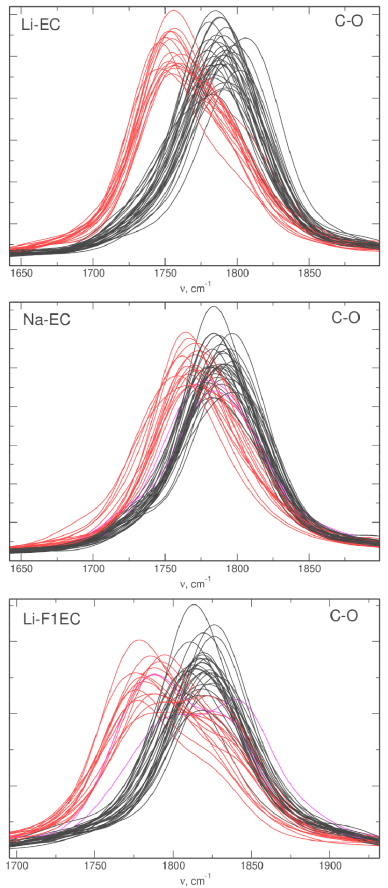
\includegraphics[width=0.4\textwidth]{img/4-ir-spectra-from-aimd-simulations/3-carbonates/ft-c-o.png}
    \singlespacing
    \caption{Fourier transforms of C=O bond lengths of solvent molecules. Free solvent molecules are black, molecules interacting with metal cations are red, and in magenta molecules interacting with the metal only during a part of MD trajectory are marked}
    \label{fig:carbonates-ft-c-o}
\end{figure}

As for previously described systems, FTs of geometrical parameters for individual solvent molecules were calculated. Example results for all of C=O bonds are shown in Figure~\ref{fig:carbonates-ft-c-o}. "Free" and bonded solvent molecules are distinguished with colors: black is used for "free" and red is used for bonded molecules. The difference between these two groups is clear: all bonded carbonates have maxima of FTs at higher frequencies than molecules interacting with cations. These separation of peaks could be related to appearance of the new band redshifted with respect to the original stretching C=O in the IR spectrum. Similarly as observed in Figure~\ref{fig:carbonates-ir-electrolytes}, the largest shifts are observed for LiTFSI in F1EC, while the smallest for NaTFSI in EC. There were also carbonate molecules, which interacted with Me$^{+}$ only within a~part of the MD trajectory and they are marked in magenta. For them shifts are also observed, but are smaller than for molecules forming complexes for the whole time of simulation.

\begin{figure}[ht]
    \centering
    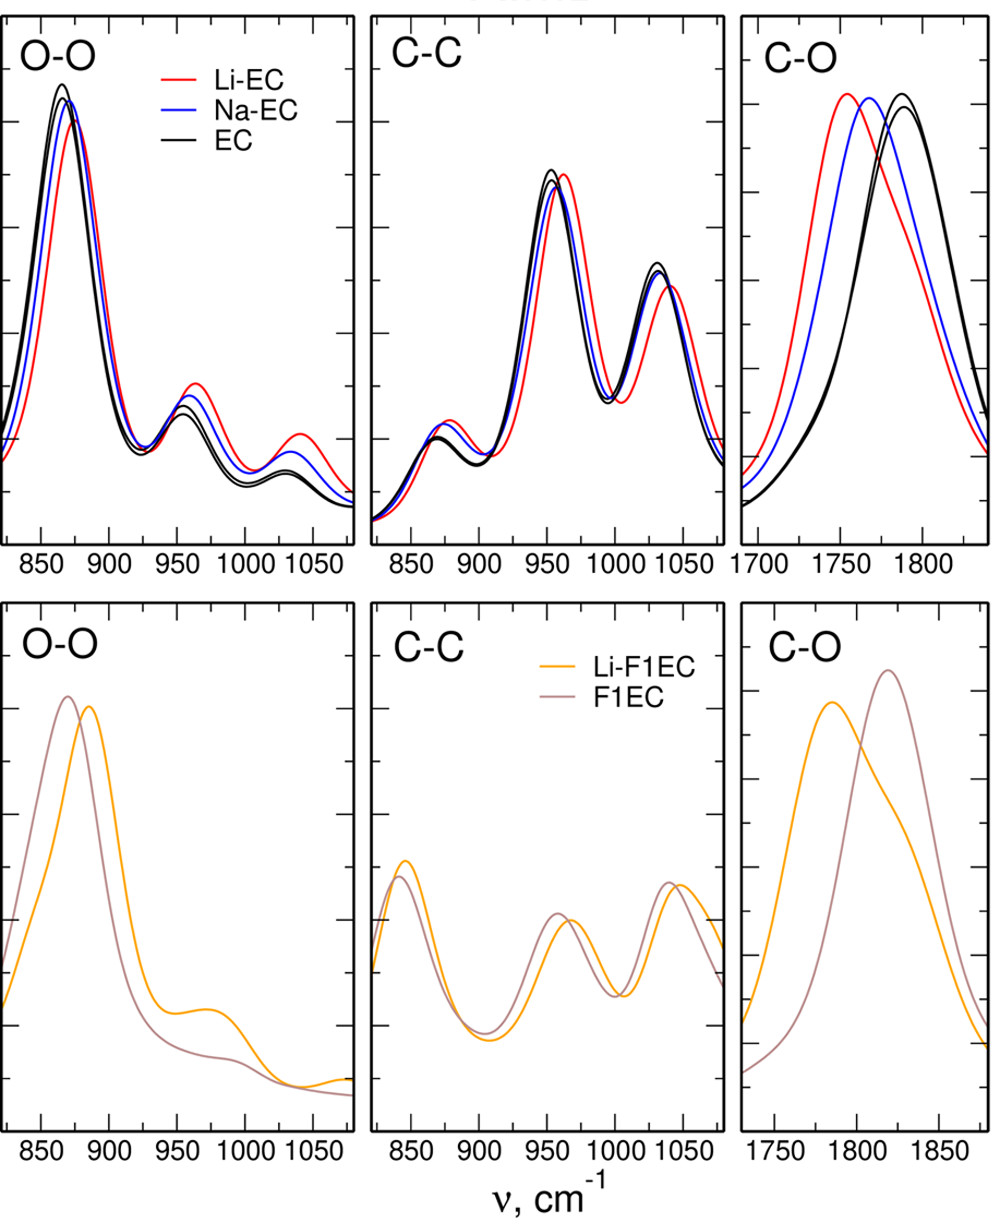
\includegraphics[width=0.4\textwidth]{img/4-ir-spectra-from-aimd-simulations/3-carbonates/ft-averages.png}
    \caption{Averaged Fourier transforms of interatomic distances}
    \label{fig:carbonates-ft-averages}
\end{figure}


Averaged FTs for geometrical parameters divided into bonded an free solvent molecules are plotted in Figure~\ref{fig:carbonates-ft-averages}. The observed shifts are comparable with those observed in IR spectra, here for C=O in EC there are shifts by 35 cm$^{-1}$ for lithium electrolyte (compared to 25~cm$^{-1}$ in IR spectrum) and 21~cm$^{-1}$ for sodium electrolyte (compared to 16~cm$^{-1}$ in IR spectrum), respectively. For LiTFSI obtained shift equals 33~cm$^{-1}$ (with 33~cm$^{-1}$ observed in the IR spectrum).


These FTs help to trace changes of local oscillations, but it is important to note that the shape of the IR spectrum depends on how these local modes couple to the global modes of the whole system and whether they change the dipole moment of the whole system. If they do not have an influence on the dipole moment, they do not carry the IR intensity, thus this analysis serves as a~tool to monitor the differences in the environment of different molecules, but is not able to directly reproduce the vibrational spectrum.

\begin{table}[ht]
\centering
\caption[Observed shifts of chosen bands in IR spectra compared to experimental values]{Observed shifts of chosen bands in IR spectra compared to experimental values, references are given for each value}
\label{tab:carbonates-experimental-comparison}
\begin{tabular}{cccc}
\toprule
Electrolyte & Vibration                                                     & AIMD shift {[}cm$^{-1}${]} & Experimental shift {[}cm$^{-1}${]} \\
\midrule
Li-F1EC     & C=O                                                           & -33                   & -30~\cite{fluorination-2}                           \\
Li-EC       & C=O                                                           & -25                   & -30~\cite{fluorination-2}, -36~\cite{vibrational-exp-3}                      \\
Na-EC       & C=O                                                           & -16                   & -20~\cite{vibrational-exp-3}                           \\
Li-F1EC     & \begin{tabular}[c]{@{}c@{}}breathing ring\\ mode\end{tabular} & +17                   & +17~\cite{neutron-diffraction}        \\
\bottomrule
\end{tabular}
\end{table}

Observed shifts of the C=O band cannot be directly compared with experimental values, because this vibration in EC was not studied in the experimental work~\cite{fluorination-2}, but data for other similar carbonate solvents are available and could be compared to results presented here. Shifts of the C=O band in 1~M LiTFSI solutions in diethyl carbonate and ethyl(fluoroethyl)carbonate are about~30~cm$^{-1}$~\cite{fluorination-2}. Another work studied spectra of electrolytes based on ethyl methyl carbonate, for NaTFSI solution observed C=O shift was equal~20~cm$^{-1}$ and for LiTFSI solution~36~cm$^{-1}$. In Raman spectrum for LiTFSI in F1EC, for the ring breathing mode a~blue shift of 17~cm$^{-1}$ was observed~\cite{neutron-diffraction}. Mentioned shifts are presented with experimental values in Table~\ref{tab:carbonates-experimental-comparison}. Thus, shifts observed for acyclic carbonates (as well as for ring breathing mode in cyclic carbonates) stay in an agreement of data obtained from AIMD and also the smaller size of the effect for sodium cation agrees with the size of experimentally observed changes. 

\cleardoublepage